%!TEX root = report.tex
\section{Echo-SLAM}

\subsection{Sine Sweep Generation}

A common signal for recording room impulse responses is the sine sweep. 
Since for the scale of the present setup, mostly low frequencies are of interest, a exponential increase of frequencies is chosen, going from$f_1=100 \text{Hz}$ to $f_2=20000 \text{Hz}$. 
\begin{equation}
    x_{exp}(i) = fac \times amp \times \sin(\frac{2 \pi f_1 N}{F_s log(\frac{f_2}{f_1})}  (e^{\frac{i}{N}log(\frac{f_2}{f_1})} - 1)) \quad \text{for $i = 0 \cdots N$}
    \label{}
\end{equation}

Where $N=T_{in}F_s$ and $F_s$ is the sampling frequency. The Fourier transform visualizes the richness of the signal in low frequencies (Figure \ref{fig:sweep_fft}) and the spectrogram gives a more intuitive visualization (Figure \ref{fig:sweep_spectrogram}).
The type chosen for the wavfile is a signed Integer of 16 bits, which can be read by \textit{PyAudio}, so the signal is amplified by $amp==2^{16-1}$ and damped with a factor of $fac=0.8$. 

To avoid a too abrupt start of which the speakers would not be capable, a hanning window is applied to the start of the signal (see Figure \ref{fig:sweep_start})

\begin{figure}[H]
	\centering		
	\begin{subfigure}[b]{0.8\linewidth}
        \centering
		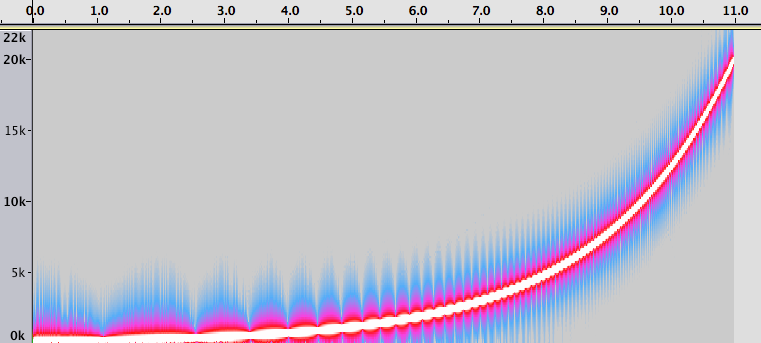
\includegraphics[width=\linewidth]{files/sweep_spectrogram.png}
        \caption{Spectogram of sine sweep}
        \label{fig:sweep_spectrogram}
	\end{subfigure} \\
	\begin{subfigure}[b]{0.49\linewidth}
        \centering
		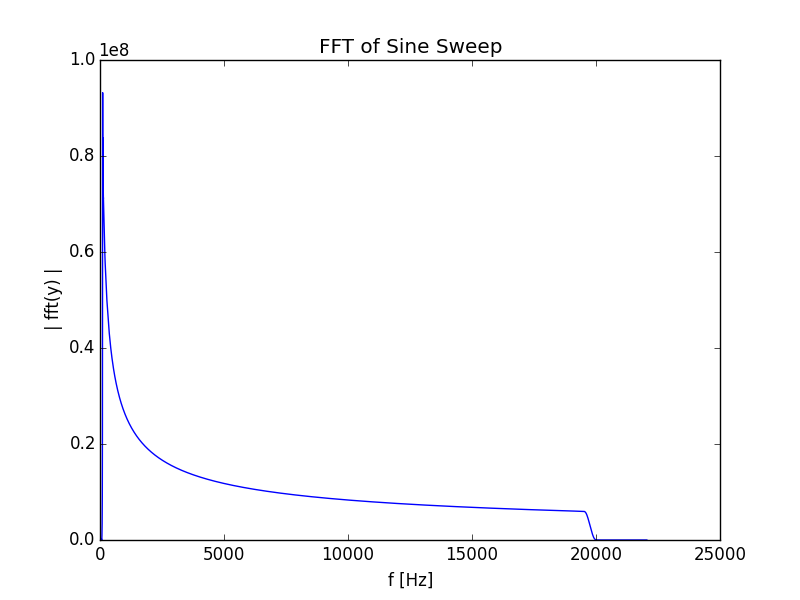
\includegraphics[width=\linewidth]{files/sweep_fft.png}
        \caption{FFT of sine sweep}
        \label{fig:sweep_fft}
	\end{subfigure}
	\begin{subfigure}[b]{0.49\linewidth}
        \centering
		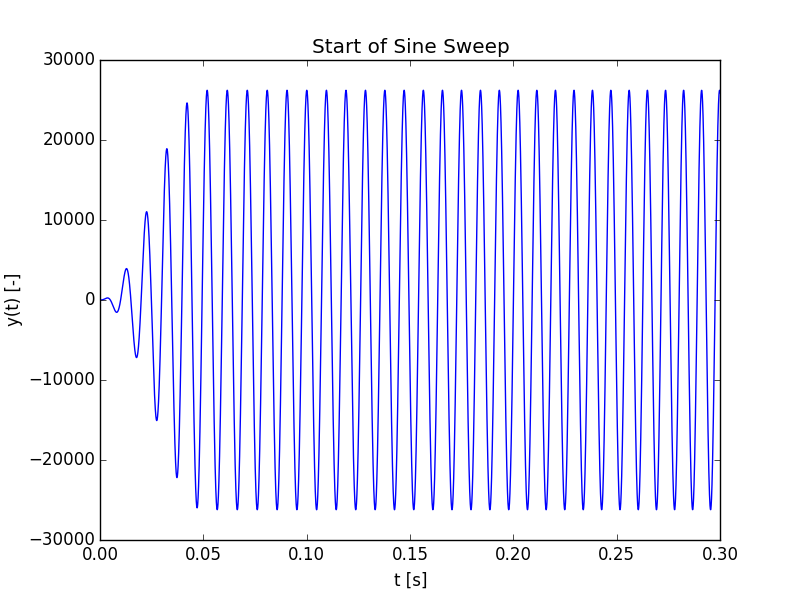
\includegraphics[width=\linewidth]{files/sweep_start.png}
        \caption{Zoom of smoothened start of sine sweep}
        \label{fig:sweep_start}
	\end{subfigure}
	\caption{Characteristics of sine sweep used for room impulse response recording} 
	\label{fig:sweep}
\end{figure}


\subsection{Recording}

The recording of the impulse response is implemented in a python script using the library \textit{PyAudio}. For a duration of $T_{out}=T_{in} + \Delta T (= 3\text{s})$, frames read from the input wav-file are sent out through the output stream and simulataneously, the data is read on the input stream. 
The incoming data can be read from multiple channels ($N_{channels}$). 
The data is stored in a matrix of size $N_{Buffers} \times (N_{Channels} \times  S_{Chunks}$ where $N_{Buffers}$ denotes the nubmer of buffers, calculated from $N_{Buffers} = \frac{T_{out} \times F_s}{S_{Chunks}}$.
%TODO: test this
The frames from the different channels are stored in alternating order and need to be \"unwrapped\" in order to store them in separate files. The resulting data matrices are single-channeled and of size $N_{Buffers} \times  S_{Chunks}$.

\subsection{Analysis}

\subsubsection{Calibration}
It is required to differentiate the delay induced by the physical distance between microphone, walls and the speakers from the delay induced by the audio system itself. Therefore an analysis of the latency of the audio system is performed. 

For this purpose, the speaker is placed at a well known position with respect to the microphone, so that the physical delay $\Delta t_i{ph}$ can be precisely calculated. 
It is then sufficient to get the total delay of the signal, $\Delta t_{tot}$ which is composed of the physical delay and the latency ($\Delta t_{tot}=\Delta t_{ph}+\Delta t_{l}$). 
The total delay is found by sending a reference signal $u_{N1}$ (in this case, a approximation of white noise) and recording the response of the microphone, $y_{N2}$. 
The white noise is generated with a randomn signal of length $T=1\text{s}$. Its histogram and fourier transform are shown in Figures \ref{fig:random_hist} and \ref{fig:random_fft} respectively. 
The power spectral density $P(k)=E(|X_N[k]|^2/N)$ of this signal should be equal to the standard deviation $\sigma^2$ if it is indeed a perfect randomn signal, meaning that its frequency is equally distributed over all frequencies. \cite{Vetterli}.
Indeed, when averaging over 1000 iterations of randomn signal generation, the obtained averaged squared magnitude, normalized by the standard variance, is close to 1 for all frequencies (see Figure \ref{fig:random_M1000}).
\begin{figure}[H]
	\centering		
	\begin{subfigure}[b]{0.49\linewidth}
        \centering
		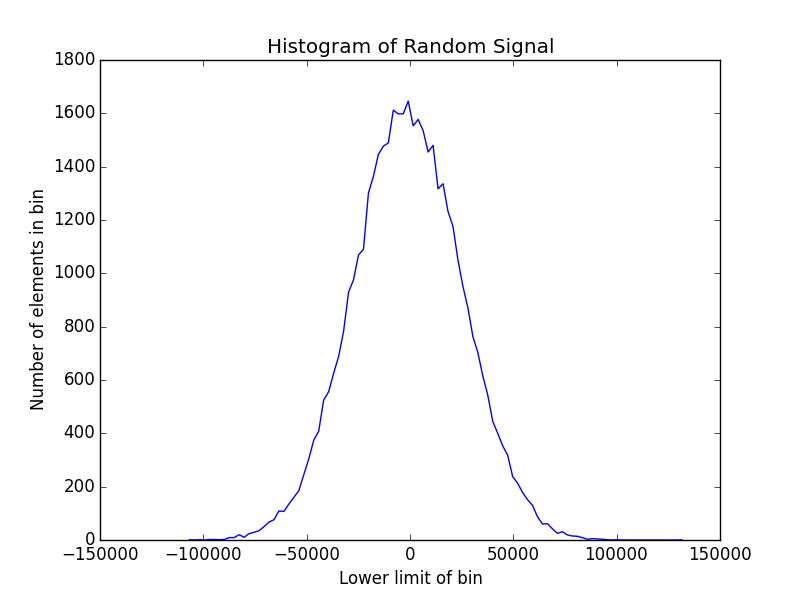
\includegraphics[width=\linewidth]{files/random_hist.png}
        \caption{Histogram}
        \label{fig:random_hist}
	\end{subfigure} 
	\begin{subfigure}[b]{0.49\linewidth}
        \centering
		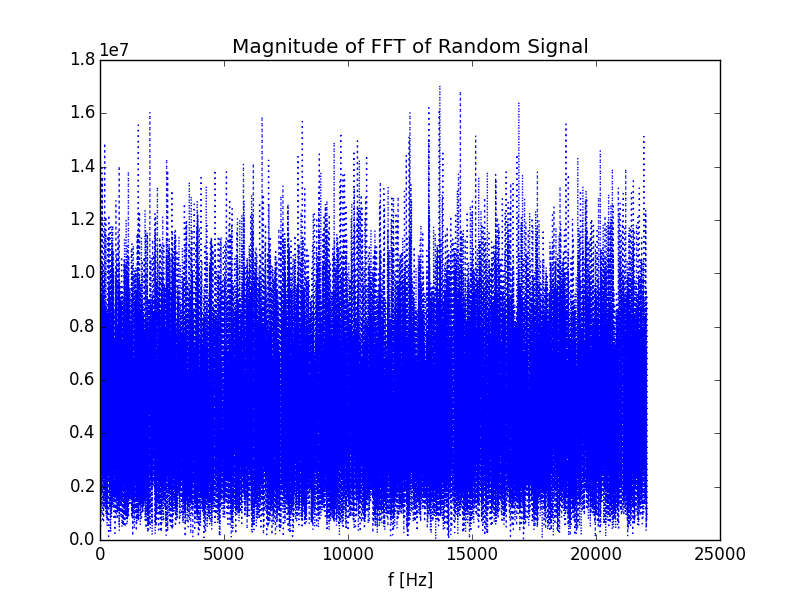
\includegraphics[width=\linewidth]{files/random_fft.png}
        \caption{Magnitude of FFT}
        \label{fig:random_fft}
	\end{subfigure}
    \begin{subfigure}[b]{0.49\linewidth}
        \centering
        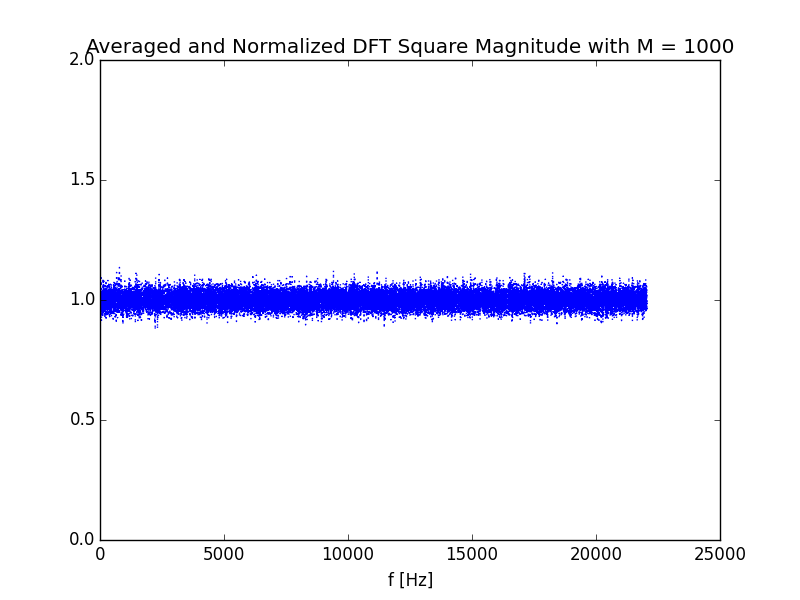
\includegraphics[width=\linewidth]{files/random_M1000.png}
        \caption{Averaged Squared Magnitude of FFT with M=1000}
        \label{fig:random_M1000}
    \end{subfigure}
	\caption{Characteristics of random signal used for calibration} 
	\label{fig:random}
\end{figure}
The response is a scaled and delayed noisy version of the input. Finding the delay comes back to laying the output signal over the input signal with different phase lags until one gets a maximum similarity. The lag corresponding to this maximum is the total delay between the input and the output. The tool that performs these steps is the cross-correlation, which, for discrete signals can be written as: 

\begin{equation}
	r_{uy}[k] = \sum\limits_{n=-\infty}^{\infty} u[n]y^*[n-k] \hspace{2em} k=0,\pm1,\pm2,...
\end{equation}

As the cross-correlation is quite computationally expensive, only the first $N_{max}$ samples of both input and output signals are correlated, which is sufficient $N_{max}$ is chosen significantly bigger than the sample index of the expected delay (for example, $N_{max}=2  \text{ s} \times F_s = 88200$)

\begin{figure}[H]
	\centering
	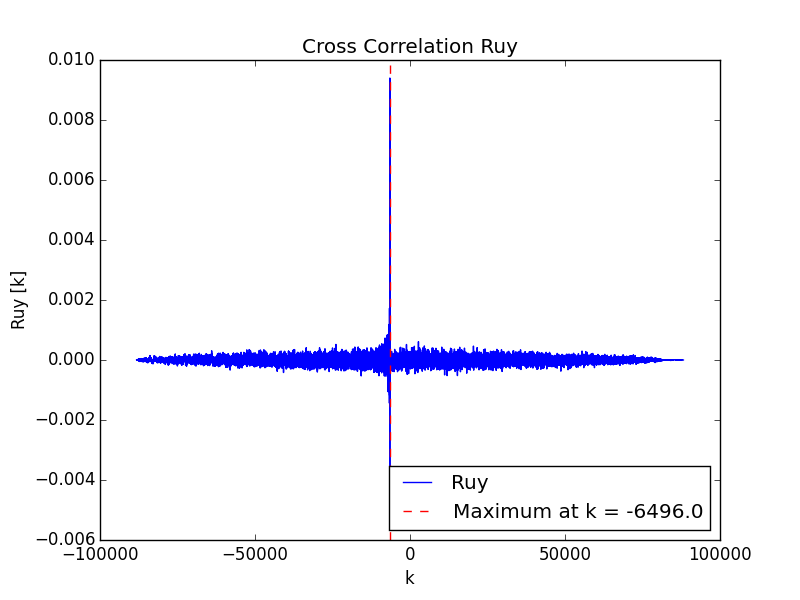
\includegraphics[width=0.6\linewidth]{files/audio_ruy.png}
	\caption{Cross correlation of white noise for latency estimation}
	\label{fig:audio_ruy}
\end{figure}

From Figure \ref{fig:audio_ruy}, one can see that the maximum occurs at sample $k_{max}=-6496$, which corresponds to a delay of $\Delta t_{tot}=k_{max}/F_s=147.3 \text{ ms}$. The distance between microphone and speaker being $d=660mm$, one finds $\Delta t_{ph} = d/c=1.9  \text{ ms}$, so the estimated latency of the sound system is about $\Delta t_{l}=145.4 \text{ ms}$.

\subsubsection{Echo SLAM}

The Room Impulse Reponses can be calculated from the frequency respose of the input $u(t)$ and of the recordet output $y(t)$ as follows:

\begin{equation}
    H(\omega) = \frac{Y(\omega)}{U(\omega)}
    \label{eq:impulse}
\end{equation}

The analysis of the impulse response is done for one specific position of the robot. For the first considerations, the microphones are assumed to be omnidirectional and placed in the exact center of the robot. 
The estimated times of arrivals can then be found from the robot position and stored in a matrix U following the notation proposed in \cite{Miranda}:

\begin{equation}
    U[n,k]=\tau_{n,k}=\frac{\| \tilde{\mathbf{s}}_{n,k}-\mathbf{r}_{n} \|}{C}=\frac{2d_{n,k}}{C}
    \label{eq:TOA}
\end{equation}

where $d_{n,k}$ denotes the distance between wall $k$ and the robot at position $n$, $\tau_{n,k}$ denotes the corresponding time of arrival and $\tilde{\mathbf{s}}_{n,k}$ and $\mathbf{r}_{n}$ denote the position of the virtual source and the robot respectively. 

These times are superimposed with the obtained impulse response to find out whether peaks occur where expected (see Figure \ref{fig:RIR_zooms}).
One can observe that there are indeed peaks around the expected times, however they are hard to differentiate from other side peaks or noise.

\begin{figure}[H]
	\centering		
	\begin{subfigure}[b]{0.49\linewidth}
        \centering
		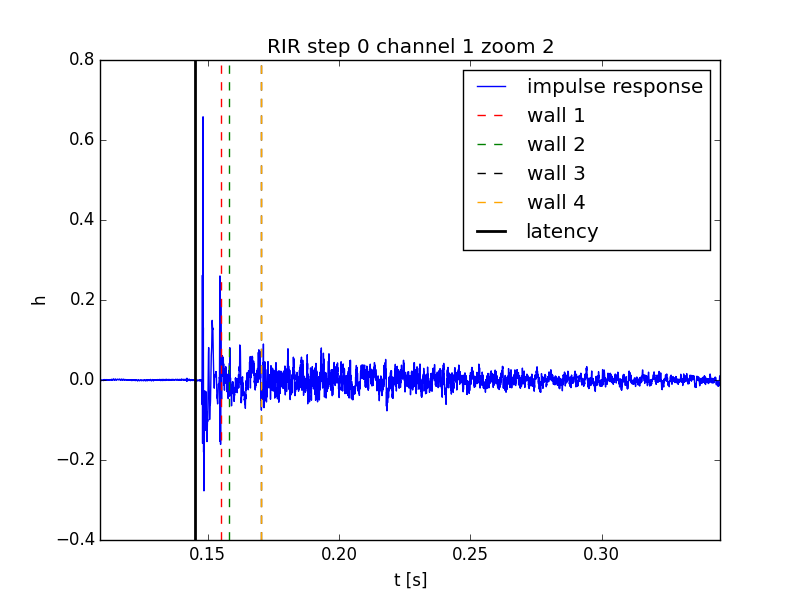
\includegraphics[width=\linewidth]{files/0_1_RIR_zoom2.png}
	\end{subfigure} 
	\begin{subfigure}[b]{0.49\linewidth}
        \centering
		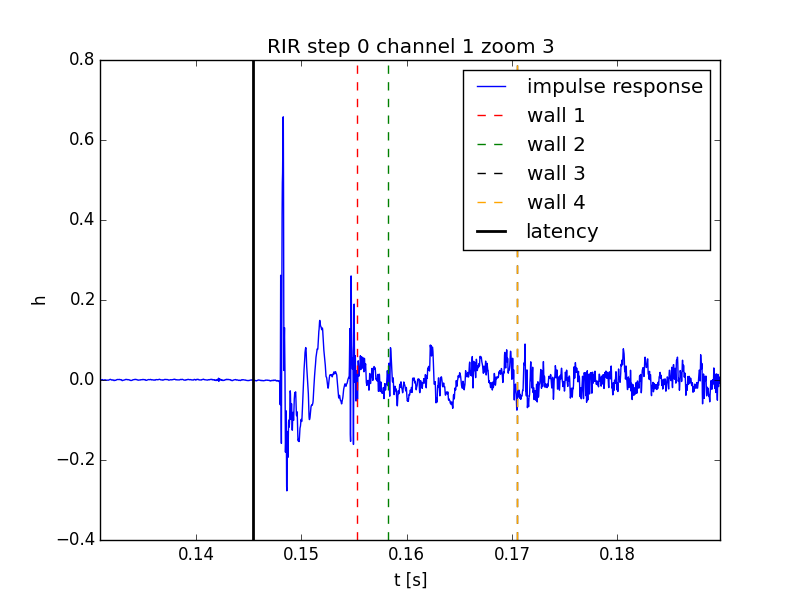
\includegraphics[width=\linewidth]{files/0_1_RIR_zoom3.png}
	\end{subfigure}
	\caption{Room impulse response with estimated times of arrival and latency time} 
	\label{fig:RIR_zooms}
\end{figure}

Looking at the frequency spectrum of the recorded response, many peaks at multiples of 108 Hz can be detected (Figure \ref{fig:RIR_filtered}, top plot). 
These peaks might be the source of unwanted noise and side peaks, which is why an attempt is done to filter them out by applying notch filters on the extraneous frequencies, trying to touch the pertinent frequencies as little as possible. A Finite Impulse Response filter (FIR) using a Kaiser Window was first implemented following \cite{Notch}, leading to few off frequency ripples and a narrow transient region. The filter is applied in forward direction and backward direction to avoid a phase shift with the filtered data. This leads to a problem too computationnally expensive in terms of memory which is not solvable by the available computers. 
The problem persists when only one forward filter is applied. 

Therefore, a more basic approach is applied, where the unwanted peaks are simply filtered out by setting the response to zero in their neighborhood. The resulting frequency response is shown in Figure \ref{fig:RIR_filtered}, bottom plot). 

\begin{figure}[H]
    \centering
    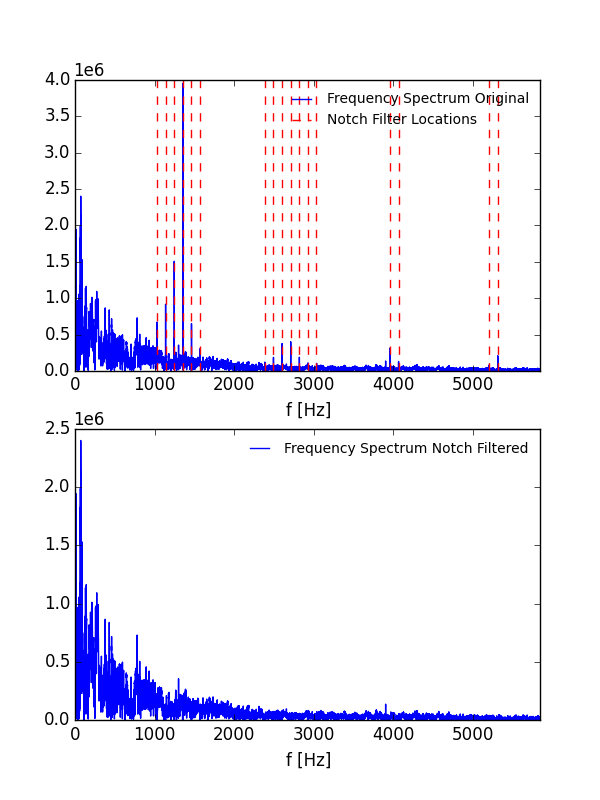
\includegraphics[width=.5\linewidth]{files/NotchY.png}
    \caption{Frequency spectrum of recorded response, unfiltered (top) and with applied Notch filter(bottom)}
    \label{fig:RIR_filtered}
\end{figure}

Unfortunately, this has no significant effect on the room imuplse response.
The reason why the walls are not well detected has to lie somehwere else. 
By construction, the robot obstructs the direct path between walls and the speaker, which could lead to unwanted early echoes and an attenuation of the wall echoes.
Another error source is that different parts of the robot and other loose part such as the speaker itself, the glass wall in the room or non removable accessories start to vibrate at their own modular frequencies.

